\documentclass{article}

% if you need to pass options to natbib, use, e.g.:
%     \PassOptionsToPackage{numbers, compress}{natbib}
% before loading neurips_2025

% The authors should use one of these tracks.
% Before accepting by the NeurIPS conference, select one of the options below.
% 0. "default" for submission
 \usepackage{neurips_2025}
 \usepackage{fontawesome}
% the "default" option is equal to the "main" option, which is used for the Main Track with double-blind reviewing.
% 1. "main" option is used for the Main Track
%  \usepackage[main]{neurips_2025}
% 2. "position" option is used for the Position Paper Track
%  \usepackage[position]{neurips_2025}
% 3. "dandb" option is used for the Datasets & Benchmarks Track
 % \usepackage[dandb]{neurips_2025}
% 4. "creativeai" option is used for the Creative AI Track
%  \usepackage[creativeai]{neurips_2025}
% 5. "sglblindworkshop" option is used for the Workshop with single-blind reviewing
 % \usepackage[sglblindworkshop]{neurips_2025}
% 6. "dblblindworkshop" option is used for the Workshop with double-blind reviewing
%  \usepackage[dblblindworkshop]{neurips_2025}

% After being accepted, the authors should add "final" behind the track to compile a camera-ready version.
% 1. Main Track
 % \usepackage[main, final]{neurips_2025}
% 2. Position Paper Track
%  \usepackage[position, final]{neurips_2025}
% 3. Datasets & Benchmarks Track
 % \usepackage[dandb, final]{neurips_2025}
% 4. Creative AI Track
%  \usepackage[creativeai, final]{neurips_2025}
% 5. Workshop with single-blind reviewing
%  \usepackage[sglblindworkshop, final]{neurips_2025}
% 6. Workshop with double-blind reviewing
%  \usepackage[dblblindworkshop, final]{neurips_2025}
% Note. For the workshop paper template, both \title{} and \workshoptitle{} are required, with the former indicating the paper title shown in the title and the latter indicating the workshop title displayed in the footnote.
% For workshops (5., 6.), the authors should add the name of the workshop, "\workshoptitle" command is used to set the workshop title.
% \workshoptitle{WORKSHOP TITLE}

% "preprint" option is used for arXiv or other preprint submissions
 % \usepackage[preprint]{neurips_2025}

% to avoid loading the natbib package, add option nonatbib:
%    \usepackage[nonatbib]{neurips_2025}

\usepackage[utf8]{inputenc} % allow utf-8 input
\usepackage[T1]{fontenc}    % use 8-bit T1 fonts
\usepackage[vietnamese]{babel} % Thêm dòng này
\usepackage{hyperref}       % hyperlinks
\usepackage{url}            % simple URL typesetting
\usepackage{booktabs}       % professional-quality tables
\usepackage{amsfonts}       % blackboard math symbols
\usepackage{nicefrac}       % compact symbols for 1/2, etc.
\usepackage{microtype}      % microtypography
\usepackage{xcolor}         % colors

\usepackage{graphicx}
\usepackage{subcaption}
\usepackage{booktabs}
\usepackage{multirow}
\usepackage{array}
\usepackage{float}
\usepackage{xcolor}
\usepackage{amsmath}

% Note. For the workshop paper template, both \title{} and \workshoptitle{} are required, with the former indicating the paper title shown in the title and the latter indicating the workshop title displayed in the footnote. 
\title{DATATHON 2026 -- The Gridbreakers (Vòng 1)\\ Nhóm: DanaScience
}


% The \author macro works with any number of authors. There are two commands
% used to separate the names and addresses of multiple authors: \And and \AND.
%
% Using \And between authors leaves it to LaTeX to determine where to break the
% lines. Using \AND forces a line break at that point. So, if LaTeX puts 3 of 4
% authors names on the first line, and the last on the second line, try using
% \AND instead of \And before the third author name.

\author{%
    \begin{tabular}{c c}
        Nguyễn Đăng Nhân$^1$ & Lê Tự Phong$^1$ \\
        Ngành Khoa học dữ liệu & Ngành Khoa học dữ liệu \\
        \texttt{dangnhan0610@gmail.com} & \texttt{phongletu78@gmail.com} \\[0.5em]
        Nguyễn Thành Bảo$^1$ & Đặng Thanh Huyền$^1$ \\
        Ngành Công nghệ thông tin & Ngành Khoa học dữ liệu \\
        \texttt{thanhbao0905@gmail.com} & \texttt{thanhhuyendang2006@gmail.com}
    \end{tabular}
    \AND
    {\small $^1$ Trường Đại học Khoa học tự nhiên, ĐHQG-HCM\\[0.4em]
    \faGithub: \href{https://github.com/nhannd2006/DATATHON2026-Vintellegence-DanaScience}{https://github.com/nhannd2006/DATATHON2026-Vintellegence-DanaScience}}
  % \And
  % Coauthor \\
  % Affiliation \\
  % Address \\
  % \texttt{email} \\
}

\definecolor{insightbox}{RGB}{232,248,240}
\definecolor{insightborder}{RGB}{45,106,79}
\definecolor{warnbox}{RGB}{255,243,205}
\definecolor{warnborder}{RGB}{230,76,51}

\newcommand{\insightbox}[1]{%
  \begin{center}
    \fcolorbox{insightborder}{insightbox}{%
      \begin{minipage}{0.93\linewidth}
        \small\textbf{$\rightarrow$ Insight:} #1
      \end{minipage}
    }
  \end{center}
}

\makeatletter
\@anonymousfalse
\makeatother


\begin{document}


\maketitle

\begin{abstract}
    Báo cáo sử dụng trực quan hóa đa tầng để nhận diện rủi ro từ nhóm khách hàng ``At Risk'' (67\%) và sự suy giảm quy mô doanh thu dù tính mùa vụ Q2 (Index 154) vẫn ổn định. Dựa trên các bằng chứng từ ma trận tồn kho và phân tích lợi nhuận, nghiên cứu đề xuất mức chiết khấu tối ưu 10\% để bảo vệ ROI. Giải pháp kỹ thuật được xây dựng trên \textbf{Hybrid Prophet-Aware Stacking} ($R^2 \approx 0{,}75$), tích hợp tối ưu hóa siêu tham số và tuân thủ nghiêm ngặt ràng buộc nhằm đảm bảo vận hành bền vững.
\end{abstract}
 
\section{Phần 2: Trực quan hóa và Phân tích Dữ liệu}
 
\subsection{Mô tả (Descriptive) — Điều gì đã xảy ra?}
 
\begin{figure}[H]
  \centering
  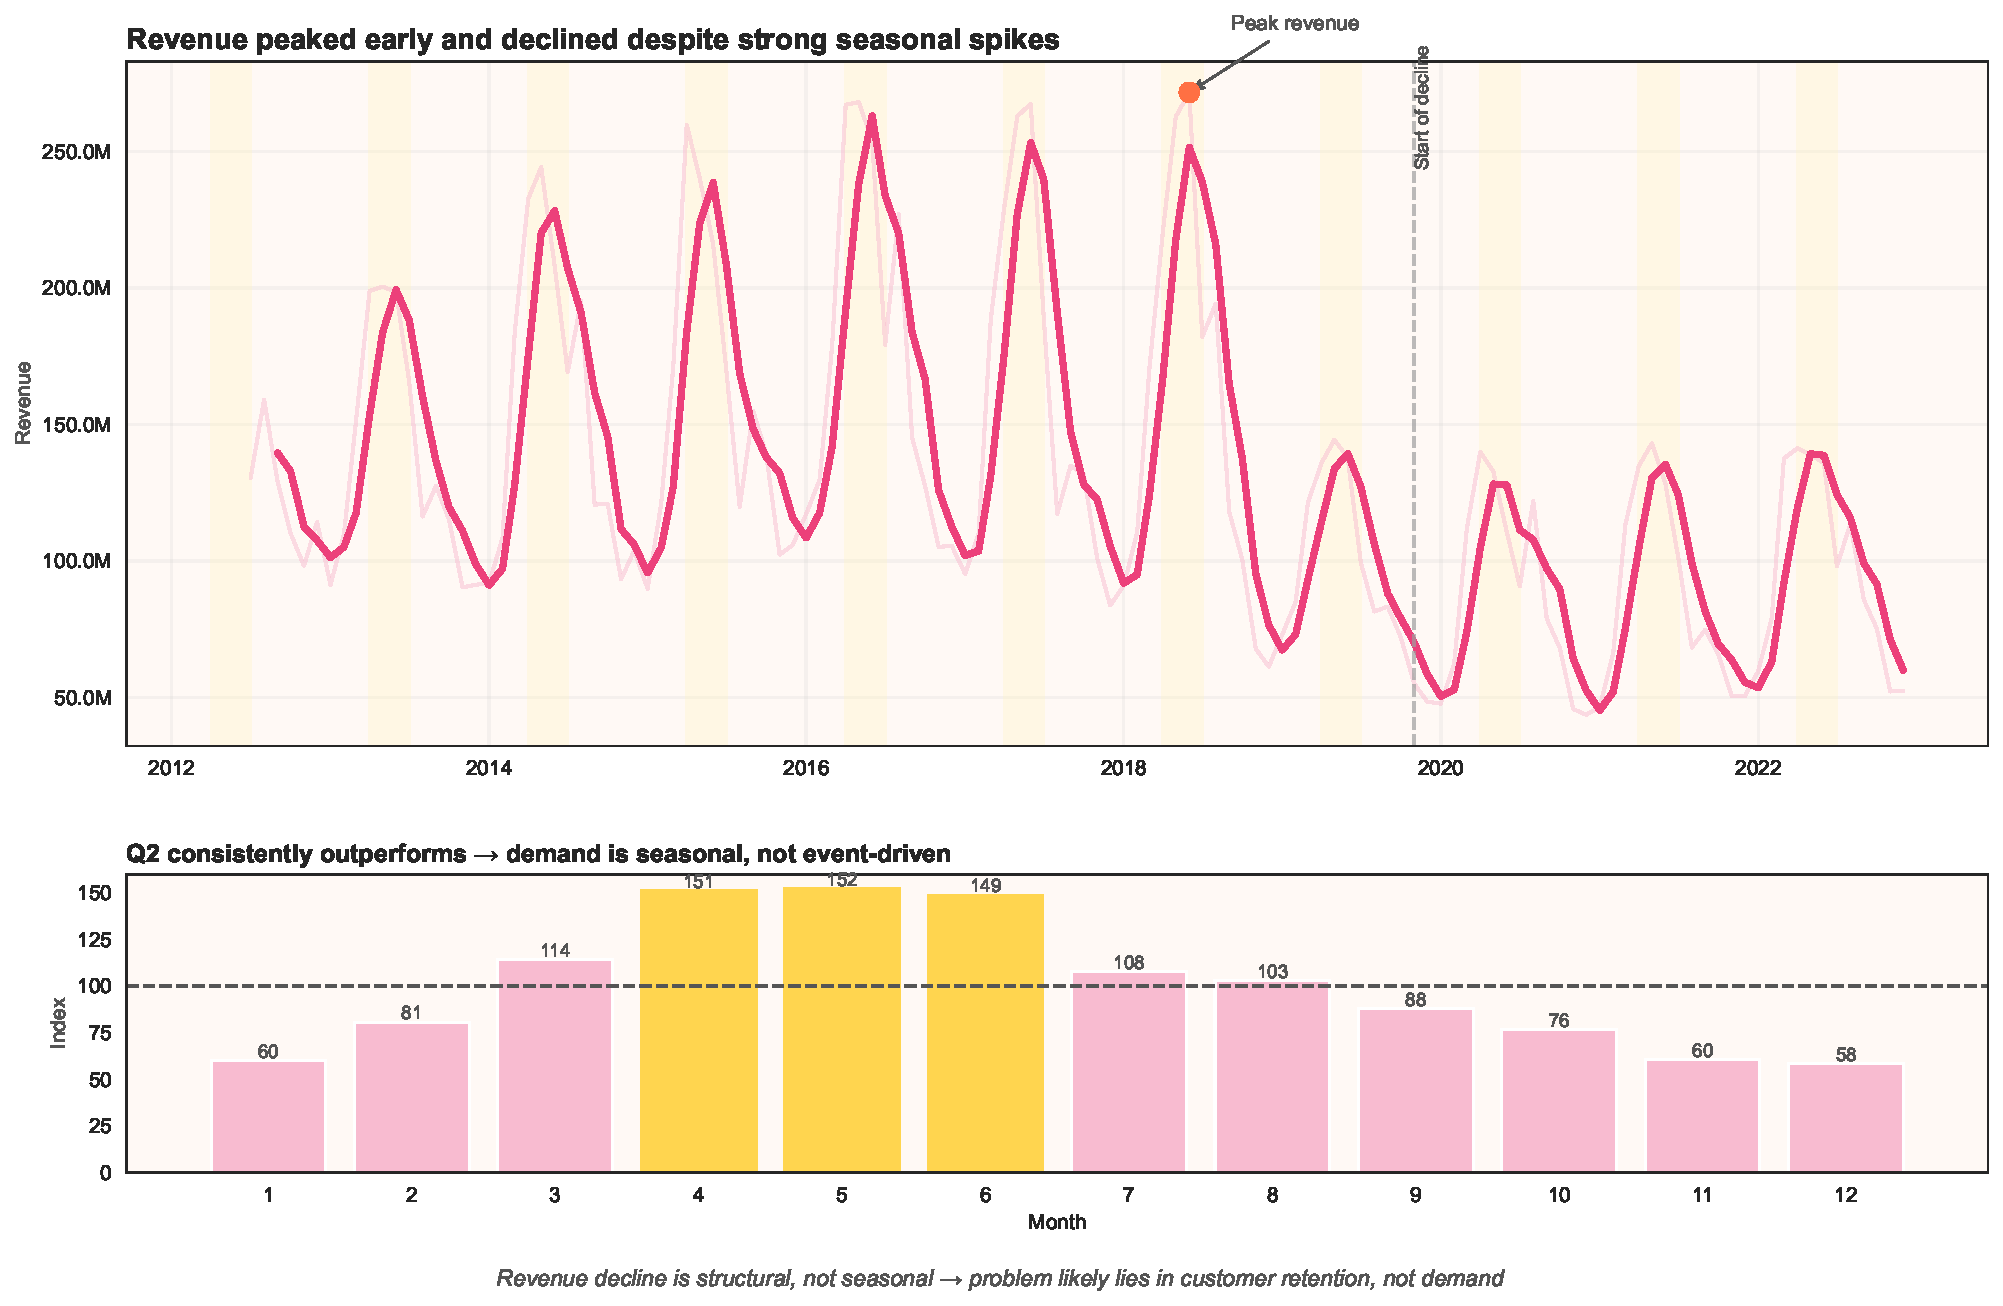
\includegraphics[width=0.8\textwidth]{../Part2/dataviz_chart1_descriptive.pdf}
  \caption{\textbf{Xu hướng Doanh thu và Chỉ số Mùa vụ (2012--2022).} \textit{Trên:} doanh thu tháng và đường làm mịn 3 tháng; vùng vàng = Q2 cao điểm. \textit{Dưới:} Chỉ số mùa vụ (Seasonality Index) với baseline = 100.}
  \label{fig:chart1}
\end{figure}
 
Doanh thu đạt đỉnh \textbf{2,10 tỷ VNĐ} (2016) rồi giảm rõ từ 2019, ổn định mức 1,04-1,17 tỷ VNĐ giai đoạn 2020-2022. Cấu trúc mùa vụ vẫn nhất quán: Q2 là đỉnh nhu cầu, tháng 5 đạt Seasonality Index \textbf{154} - gấp 2,6 lần tháng 12 tuy nhiên quy mô các đỉnh đang thu hẹp dần qua từng năm.
 
\insightbox{Sự suy giảm doanh thu không nằm ở nhu cầu thị trường (vì Q2 ổn định và dự báo được) mà có thể đến từ việc doanh nghiệp \textbf{không giữ được khách hàng} hoặc chưa bù đắp đủ lượng khách đã mất.}
 
\subsection{Chẩn đoán (Diagnostic) — Tại sao nó xảy ra?}
 
\begin{figure}[H]
  \centering
  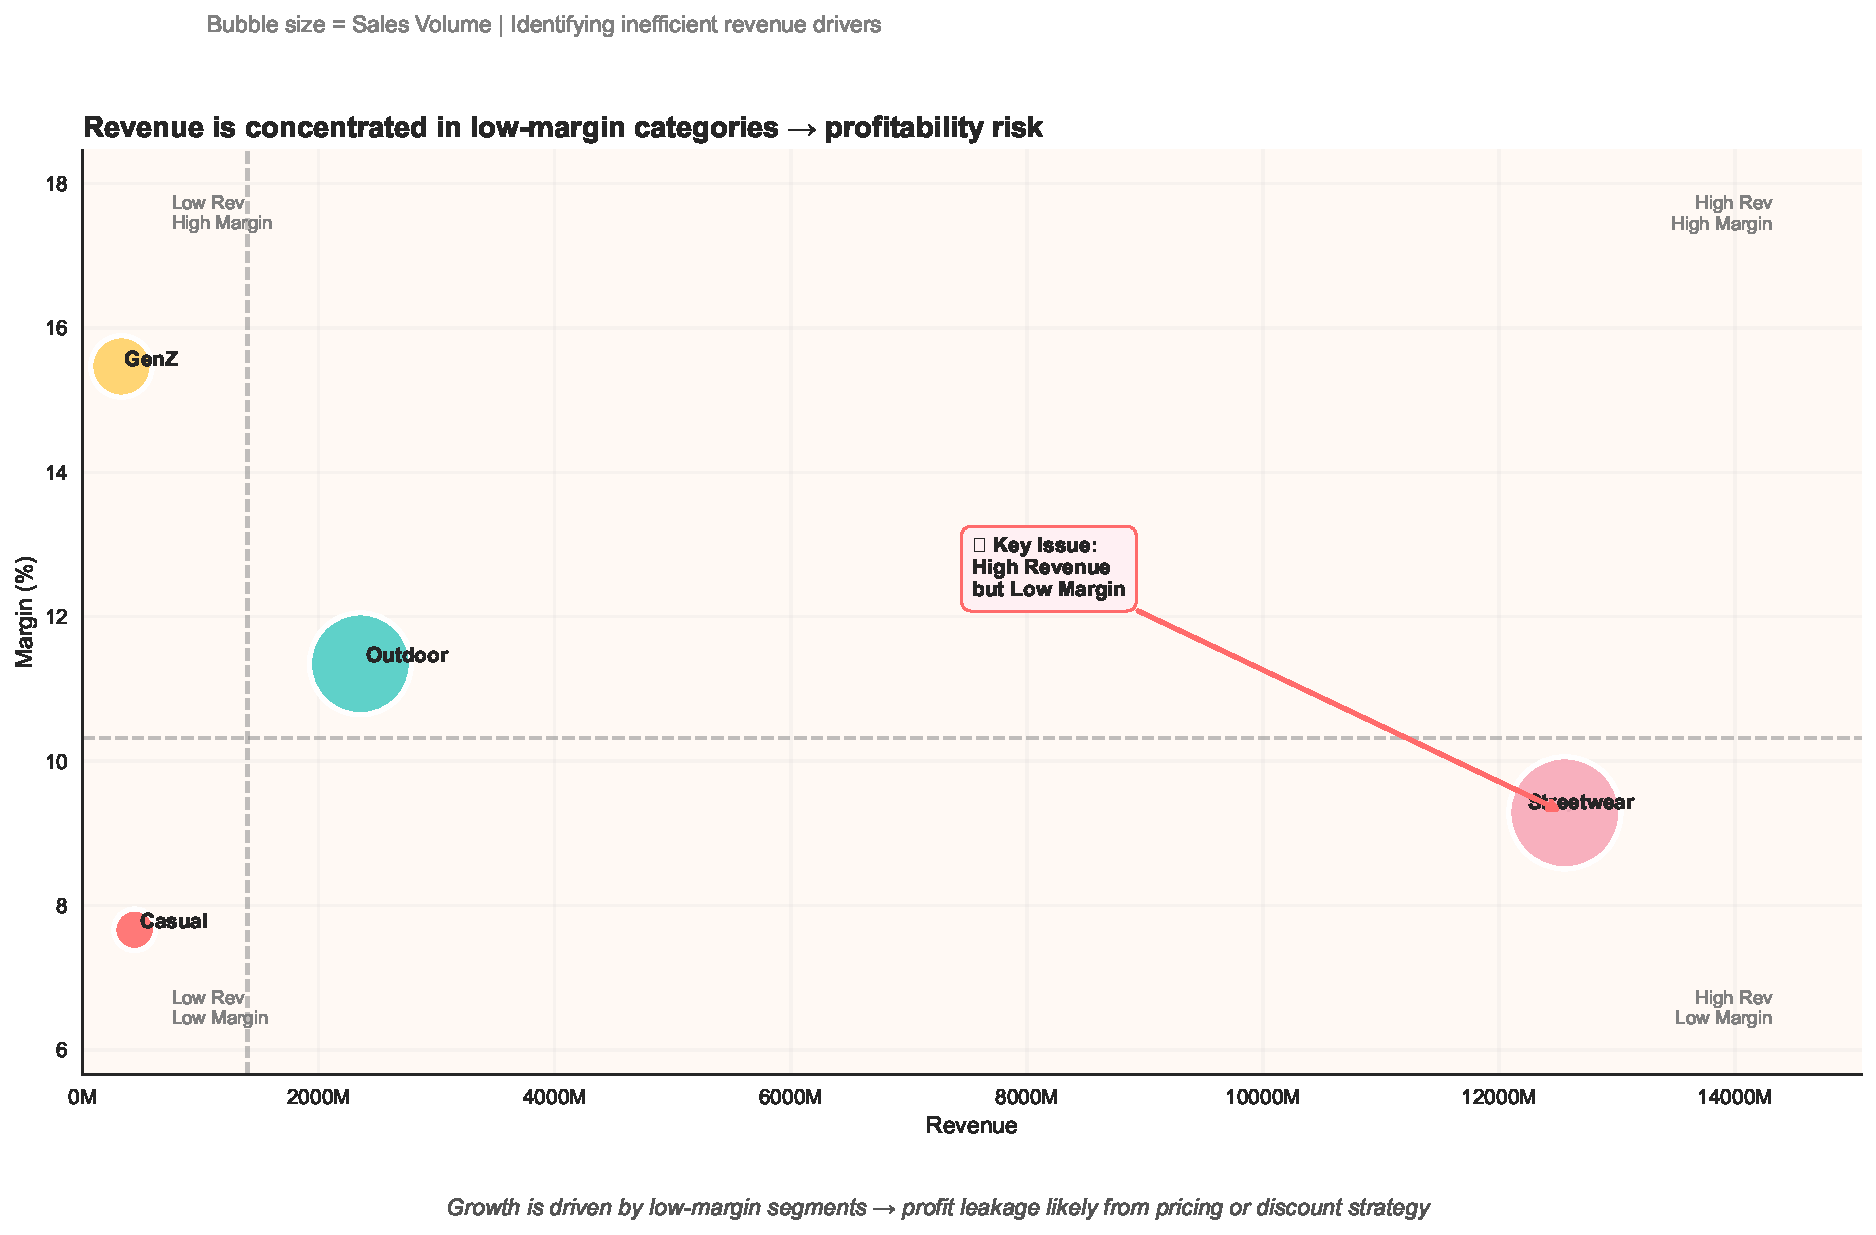
\includegraphics[width=0.7\textwidth]{../Part2/dataviz_chart2_diagnostic.pdf}
  \caption{\textbf{Ma trận tương quan doanh thu và biên lợi nhuận gộp theo danh mục sản phẩm.} (kích thước bubble tỷ lệ thuận với sản lượng bán)}
  \label{fig:chart2}
\end{figure}
 
\textbf{Streetwear} chiếm 79,9\% doanh thu nhưng có biên lợi nhuận thấp nhất (13,2\%), chỉ đóng góp 76,7\% lợi nhuận. Ngược lại, nhóm \textbf{GenZ} đạt margin cao nhất (19,1\%) dù tỷ trọng mới ở mức 2,1\%, mở ra dư địa dịch chuyển cơ cấu sang nhóm sản phẩm giá trị cao hơn.

 
\begin{figure}[H]
  \centering
  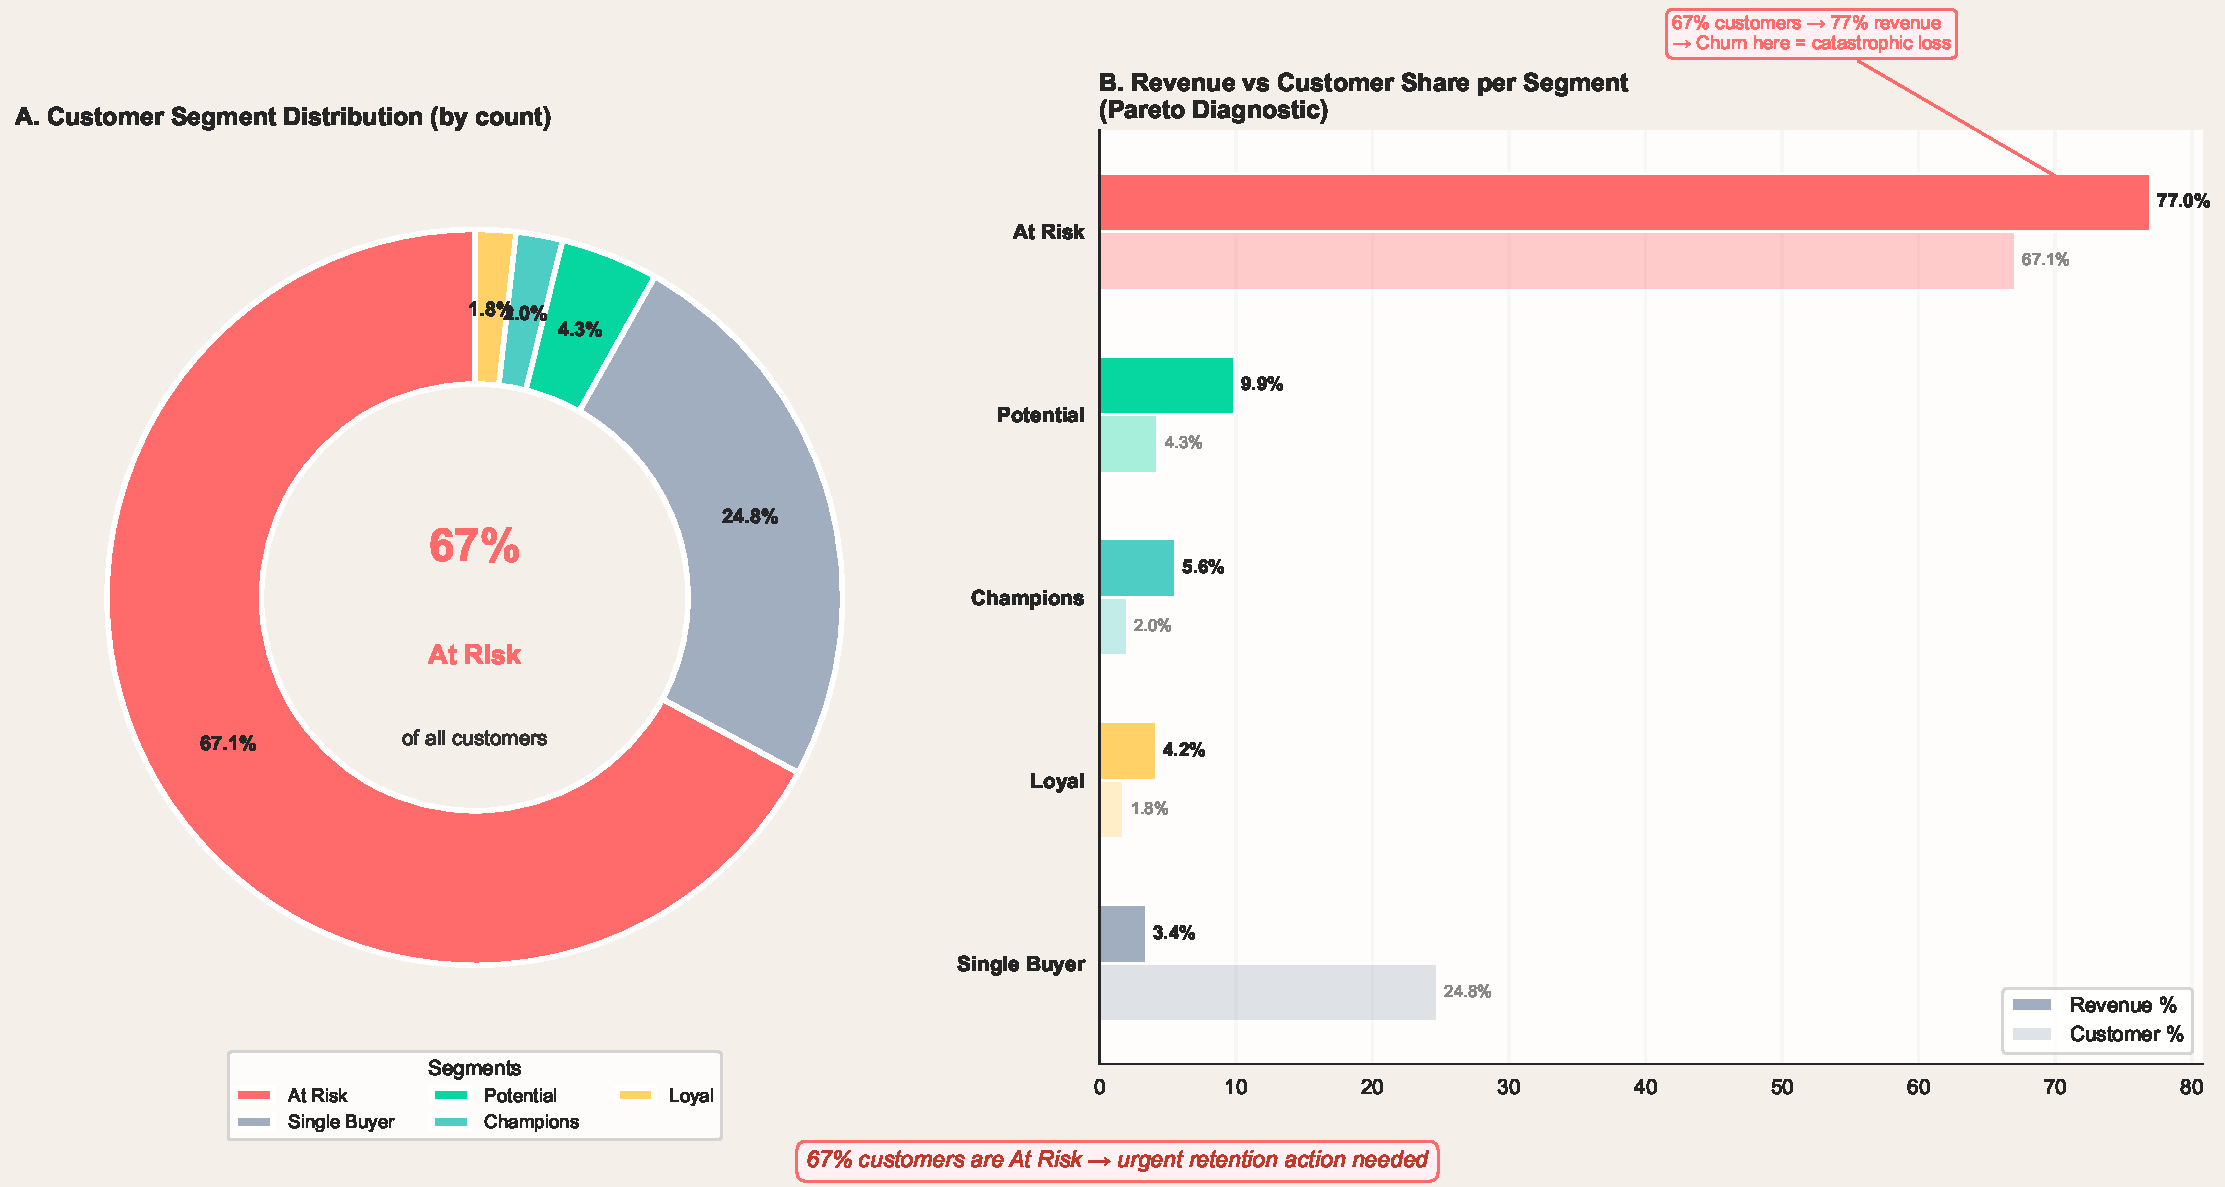
\includegraphics[width=0.8\textwidth]{../Part2/dataviz_chart3_diagnostic.pdf}
  \caption{\textbf{Phân tích sức khỏe khách hàng và Tỷ trọng doanh thu theo mô hình RFM.} Trái: phân bổ khách hàng theo phân khúc. Phải: so sánh \% đóng góp doanh thu và \% số lượng khách hàng.}
  \label{fig:chart3}
\end{figure}
 
Phân tích RFM (Recency - Frequency - Monetary) chỉ ra rủi ro tập trung cực lớn: nhóm \textbf{At Risk} (67\% khách hàng) đóng góp tới 77\% doanh thu. Với tỷ lệ khách mua một lần cao (24,8\%) và nhóm trung thành chỉ vỏn vẹn 3-4\%, bài toán then chốt của doanh nghiệp là năng lực giữ chân khách hàng thay vì chỉ tập trung thu hút mới.
 
\insightbox{(1) Streetwear kéo biên lợi nhuận xuống dù dẫn đầu doanh thu; (2) 67\% khách hàng đang ``At Risk'' và kiểm soát 77\% doanh thu --- mất nhóm này là mất phần lớn doanh nghiệp.}
 
\subsection{Dự báo (Predictive) - Điều gì có thể xảy ra?}
 
\begin{figure}[H]
  \centering
  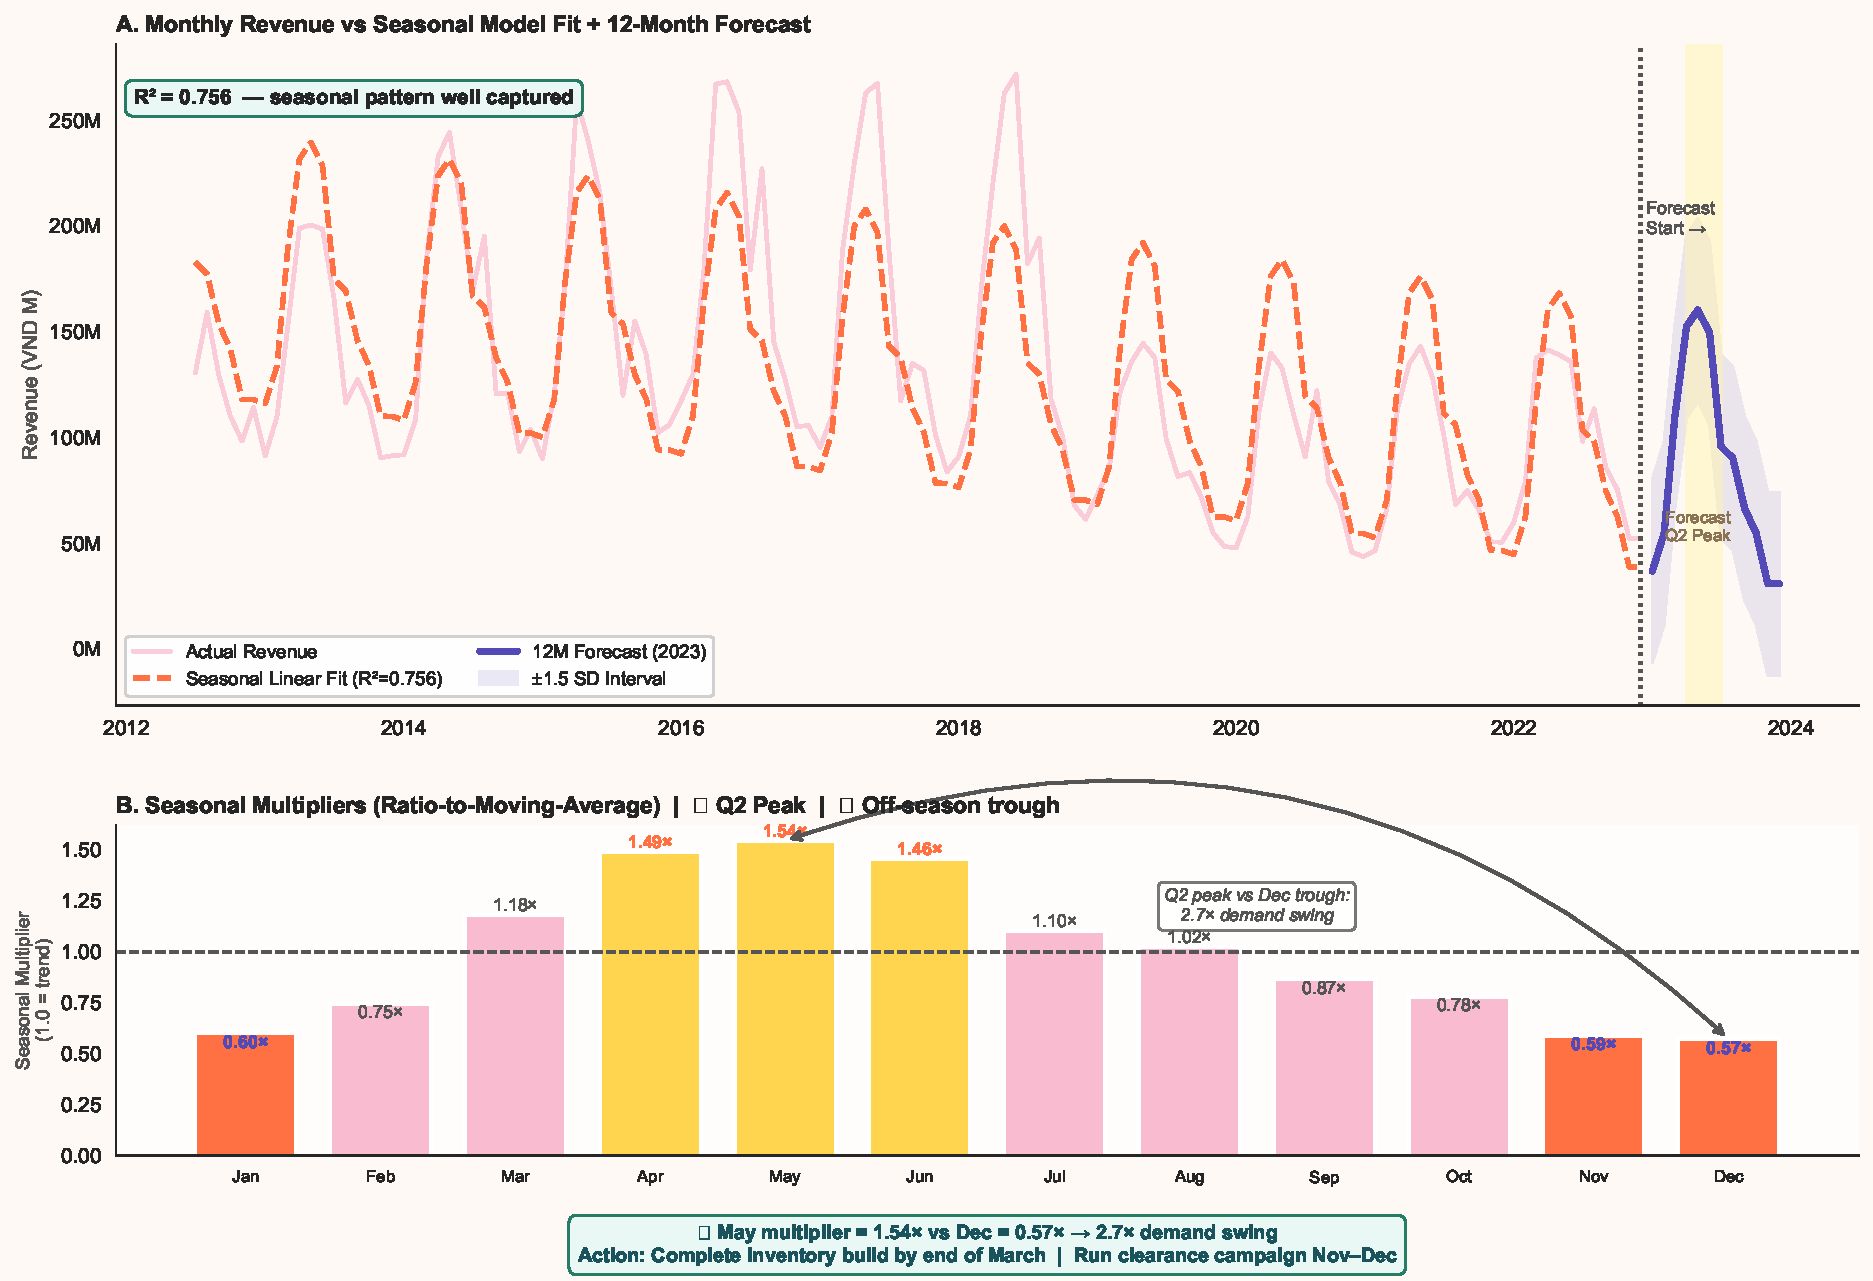
\includegraphics[width=0.7\textwidth]{../Part2/dataviz_chart4_predictive.pdf}
  \caption{\textbf{Phân rã thành phần chu kỳ và Dự báo doanh thu trong 12 tháng tới.} \textit{Trên:} doanh thu thực tế ($R^2{=}0{,}756$) và khoảng dự báo. \textit{Dưới:} hệ số mùa vụ (Seasonal Multiplier) theo từng tháng.}
  \label{fig:chart5}
\end{figure}
 
Mô hình hồi quy đạt $R^2 = 0{,}756$ xác nhận Q2 có thể dự báo với độ tin cậy cao. Với biên độ dao động \textbf{2,7×} giữa đỉnh tháng 5 (multiplier \textbf{1,54×}) và đáy tháng 12 (\textbf{0,60×}), tăng trưởng hiện tại phụ thuộc chặt chẽ vào mùa vụ trong khi xu hướng nền đang giảm nhẹ từ sau năm 2016.
 
\insightbox{Nhu cầu Q2 ổn định và dự báo được. Cần hoàn tất tích lũy tồn kho trước cuối tháng 3 để đón đỉnh tháng 5; triển khai các chương trình xả kho (clearance) vào tháng 11-12 khi nhu cầu chạm đáy.}
 
\subsection{Đề xuất (Prescriptive) - Chúng ta nên làm gì?}
 
\begin{figure}[H]
  \centering
  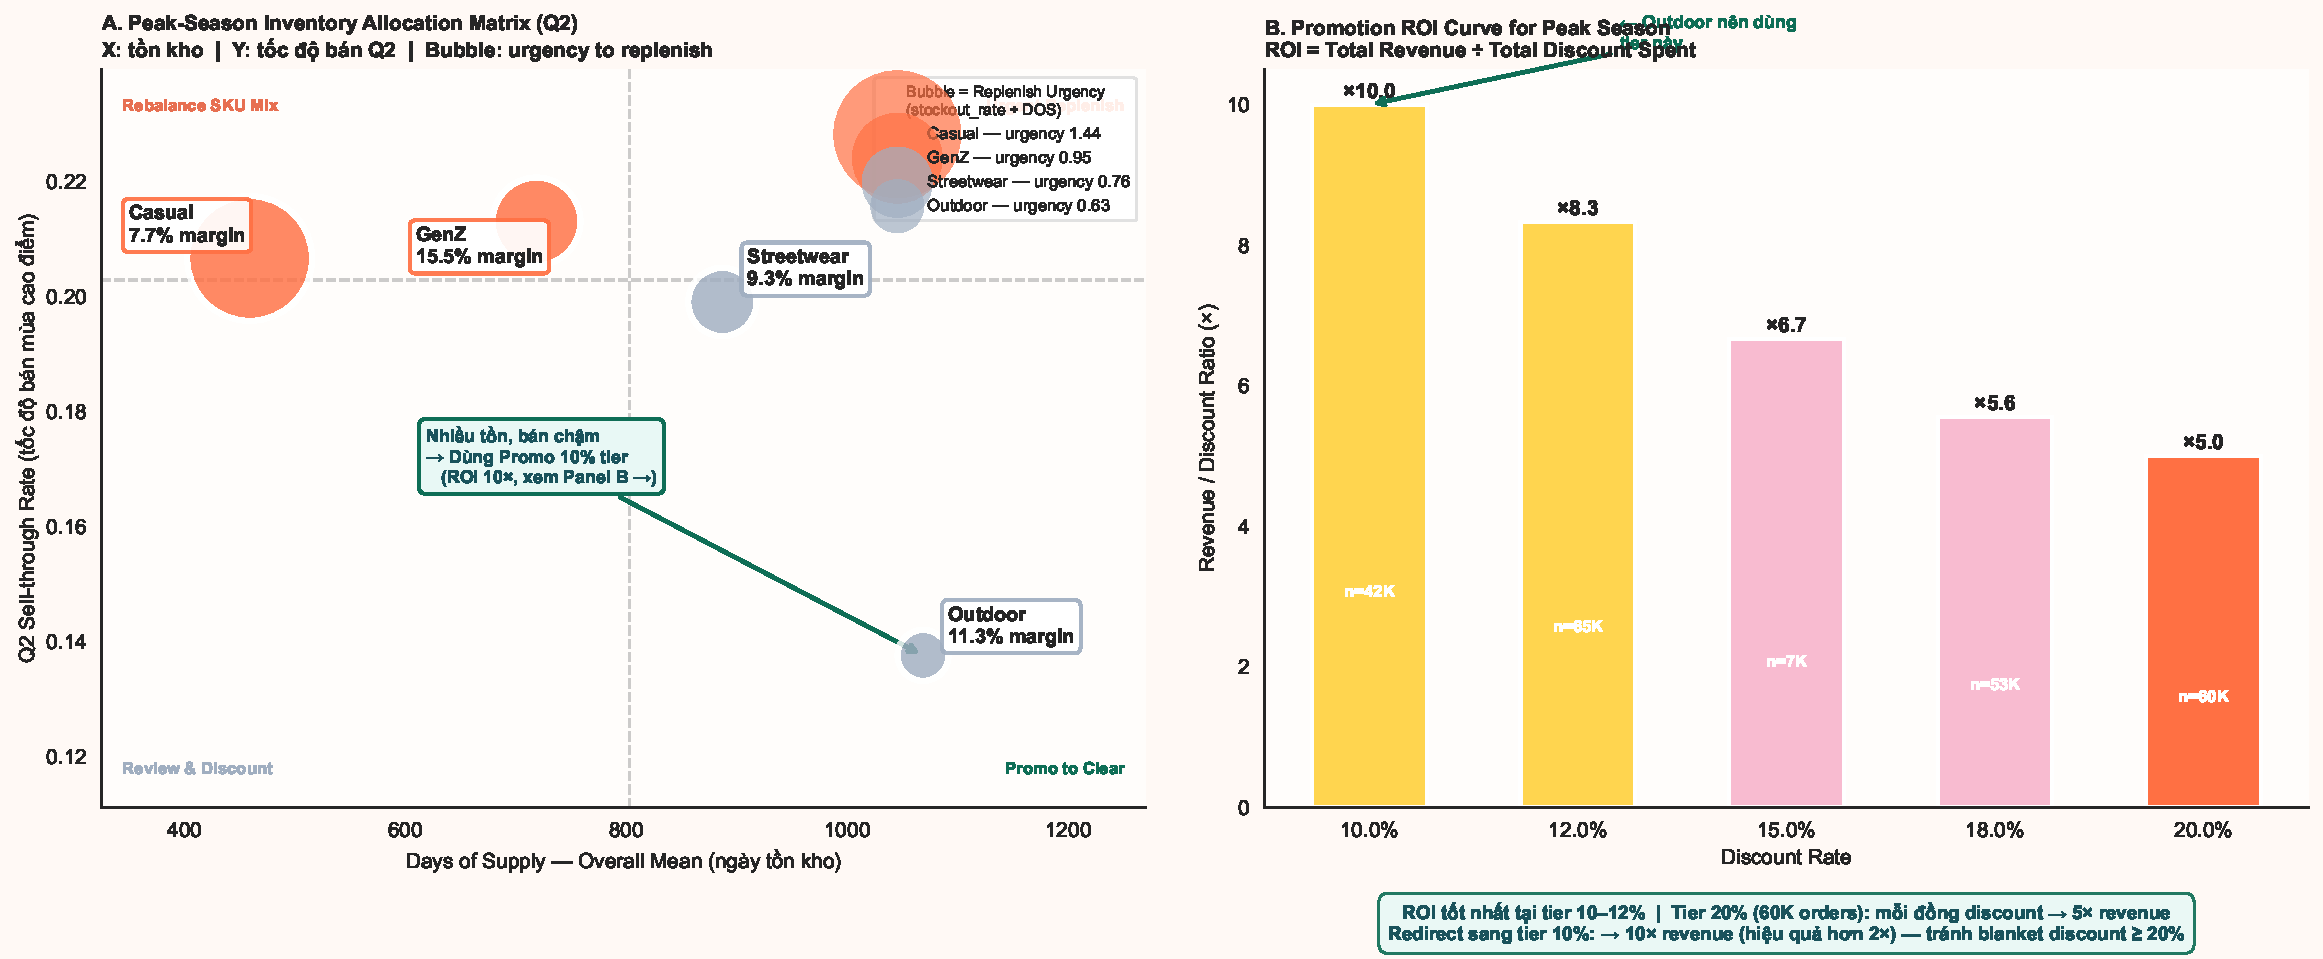
\includegraphics[width=0.8\textwidth]{../Part2/dataviz_chart5_prescriptive.pdf}
  \caption{\textbf{Ma trận tối ưu hóa Tồn kho và Đường cong hiệu quả (ROI) Khuyến mãi.} \textit{Trái:} ma trận giữa số ngày tồn kho và tỷ lệ bán hết; \textit{Phải:} phân tích tỷ lệ ROI theo từng mức chiết khấu.}
  \label{fig:chart6}
\end{figure}

Dựa trên ma trận phân bổ, nhóm \textbf{Casual} (urgency \textbf{1,44}) cần được bổ sung hàng ngay lập tức để tránh đứt gãy cao điểm; ngược lại, \textbf{Outdoor} là ưu tiên xả kho do tồn kho lên tới \textbf{1.069 ngày}. Phân tích ROI (Return on Investment) xác nhận mức chiết khấu tối ưu là \textbf{10\%} (ROI $\times$10,0) $\rightarrow$ việc duy trì mức 20\% cho 60.000 đơn hàng hiện tại đang gây lãng phí biên lợi nhuận đáng kể.
 
\insightbox{\textbf{<Kế hoạch hành động Q2>} (1) Ưu tiên bổ sung hàng (Replenish) Casual trước - mức độ khẩn cấp cao nhất; (2) Promo 10\% cho Outdoor để giải phóng 1.069 ngày tồn kho với ROI $\times$10; (3) Giới hạn mọi discount $\leq 12\%$ vì vượt ngưỡng này ROI giảm một nửa dù doanh số có thể tăng ngắn hạn.}

\section{Phần 3: Dự báo doanh thu}
\subsection{Tổng quan pipeline của mô hình}
\textbf{Kiến trúc mô hình:} Sử dụng hệ thống Hybrid Stacking: Prophet đảm nhận dự báo xu hướng và tính mùa vụ (baseline), trong khi  XGBoost, LightGBM, CatBoost tập trung dự báo phần dư (residual). Kết quả được tổng hợp qua HuberRegressor trên thang đo $\log$ cho cả Revenue và tỷ lệ COGS.

\textbf{Nhóm đặc trưng (Features):} Hệ thống đặc trưng đa dạng bao gồm dữ liệu thời gian, khoảng cách đến các đỉnh doanh thu, tín hiệu khuyến mãi (xung suy giảm theo hàm mũ, mật độ, xác suất lịch sử) và các thành phần tương tác từ mô hình Prophet.

\textbf{Quy trình huấn luyện:} Áp dụng Walk-forward CV với 4-fold (giai đoạn 2019–2022) để đảm bảo tính thực tế theo thời gian. Siêu tham số được tối ưu hóa tự động bằng Optuna trước khi huấn luyện lại trên toàn bộ tập dữ liệu huấn luyện.

\subsection{Các yếu tố dẫn động đến doanh thu (Key Drivers)}
\begin{figure}[H]
  \centering
  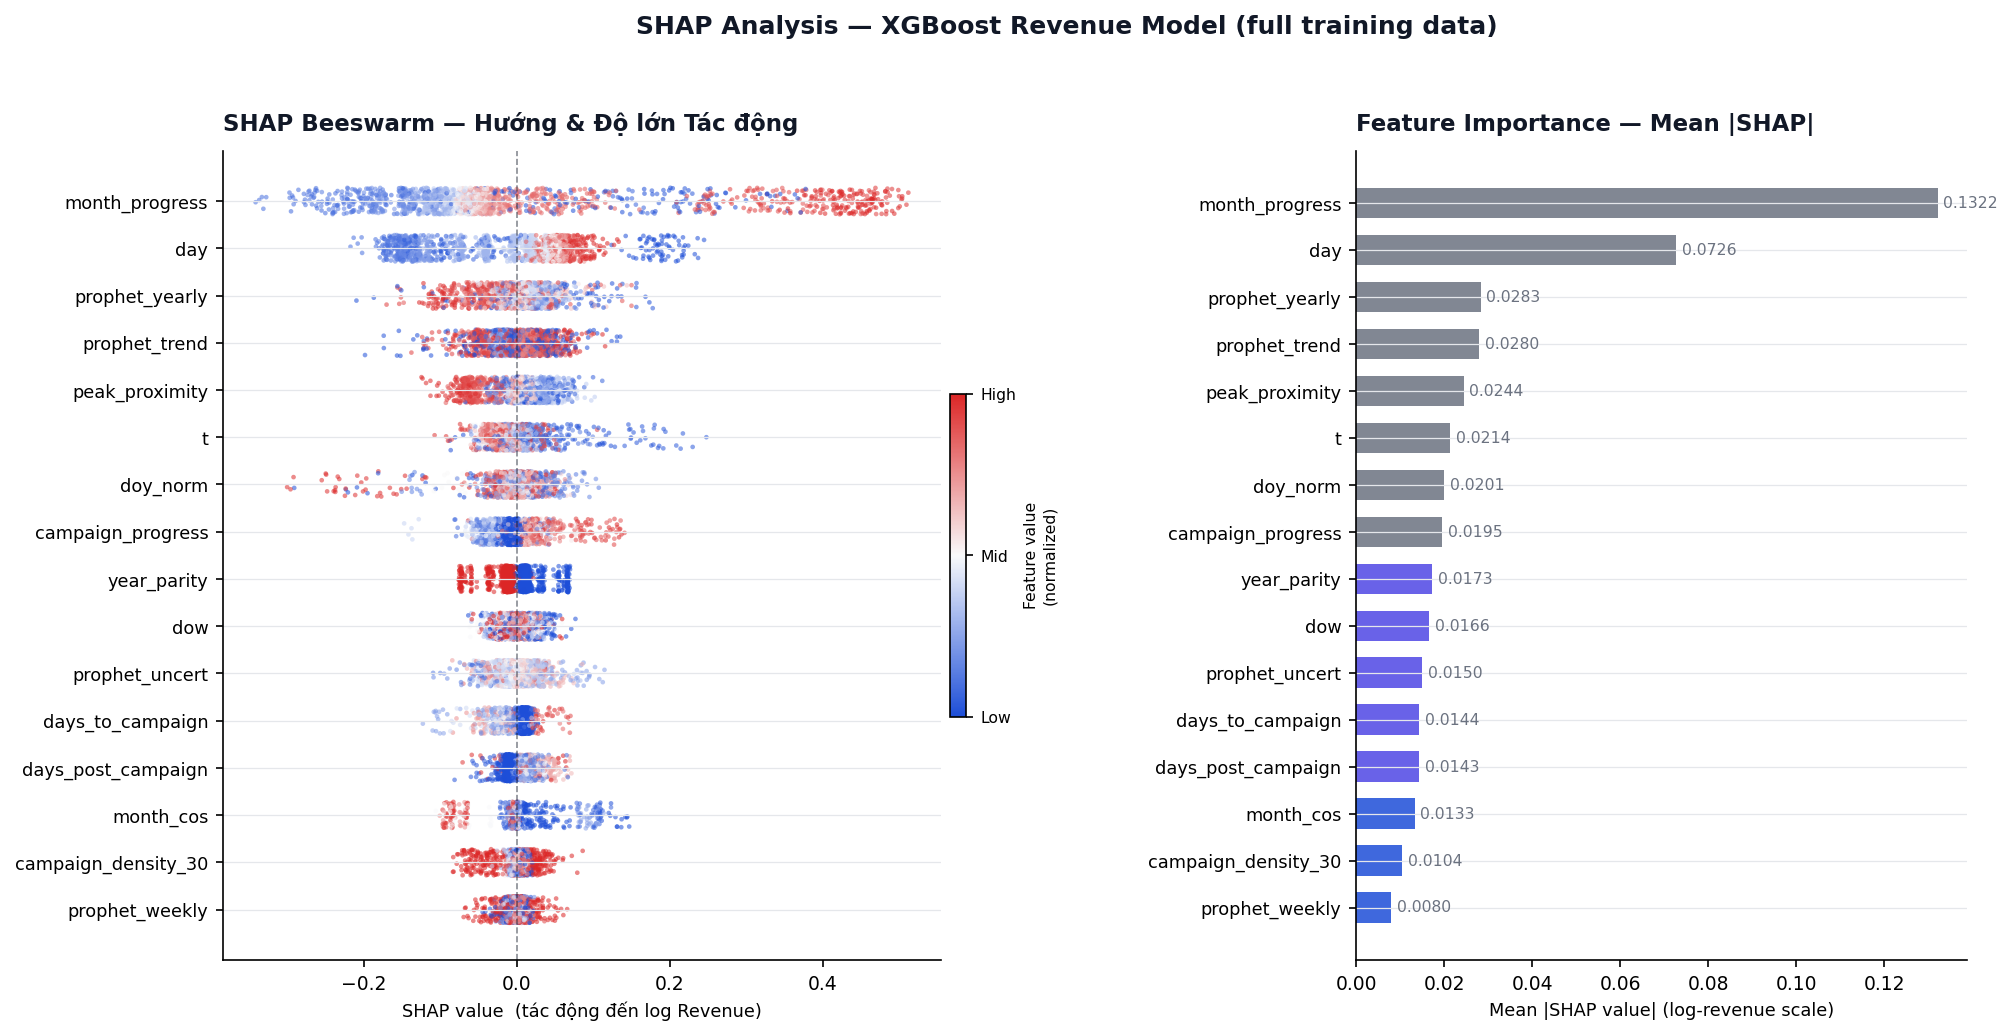
\includegraphics[width=0.8\textwidth]{../Part3/salesstack_fig2.png}
  \caption{Các yếu tố quan trọng tác động đến doanh thu dựa trên phân tích SHAP và Feature Importance.}
  \label{fig:chart5}
\end{figure}
\textbf{Tiến độ thời gian:} Doanh thu có chu kỳ lặp lại mạnh mẽ theo ngày trong tháng và vị trí trong năm.

\textbf{Hiệu ứng Campaign Kernels:}
\begin{itemize}
    \item Pre-campaign: Khách hàng có xu hướng dồn đơn ngay trước khi khuyến mãi bắt đầu.
    \item Post-campaign: Doanh thu không giảm ngay lập tức mà có độ trễ, duy trì khoảng 22\% tín hiệu sau 30 ngày.
\end{itemize}

\textbf{Sự cộng hưởng (Interaction):} Biến \texttt{campaign\_x\_peak} cho thấy hiệu quả khổng lồ khi các đợt giảm giá trùng với đỉnh mùa vụ.

\subsection{Hiệu suất và độ tin cậy}
\textbf{Độ chính xác:} Mô hình đạt $R^2 \approx 0.75$, một con số rất ấn tượng cho dữ liệu doanh thu hàng ngày có độ nhiễu cao.

\textbf{Khả năng kháng nhiễu:} Việc sử dụng hàm mất mát Huber giúp mô hình không bị "lệch hướng" bởi các ngày có doanh số tăng đột biến quá mức.

\textbf{Kiểm soát rủi ro:} Biến \texttt{prophet\_uncert} giúp mô hình tự điều chỉnh khi dữ liệu đầu vào có dấu hiệu bất thường, tăng độ an toàn cho dự báo.

\end{document}